\section{Deployment}
\begin{justify}
    As the part of the software development lifecycle that is responsible for making a software system accessible to end users, the deployment phase plays an essential role in the overall process. The effective installation, setup, and functioning of the application are the key objectives of this phase, which aims to guarantee that these objectives are met. It is important to have effective oversight in place in order to guarantee accurate application deployment.

    \vspace{0.25cm}
    \newendline Both the backend and the frontend of the Student Talent Development Center (STDC) Web Application were given significant attention during the deployment process, which followed a two-pronged strategy. A cloud-based platform was selected for each component so that it could meet the requirements for scalability, stability, and simplicity of maintenance. During the early stages of the project, it was decided to deploy the backend, which was developed with the Ruby on Rails framework. This was done in order to make communication with the API easier. On the other hand, the frontend was not deployed until the very last step, which was when the application was finally ready for production. This strategy was founded on the reality that the API was not dependent on the frontend in any manner, but rather that the client was solely dependent on the backend.
    
    \vspace{0.25cm}
    \newendline Now that we have everything out of the way, let's take a more straightforward look at the deployment process.\\
\end{justify}


\subsection{Backend Deployment (API)}
\begin{justify}
    Heroku is a cloud platform as a service that supports a number of programming languages, one of which being Ruby. The backend of the STDC Web Application was developed with Ruby on Rails, and it was deployed on Heroku. When it comes to delivering web apps, Heroku offers a platform that is both reliable and expandable.
    
    \vspace{0.25cm}
    \newendline The process of deployment consisted of the following stages:
\clearpage
    \begin{itemize}
        \item Setting up the Ruby environment, configuring the database, and making any necessary adjustments to the configurations came first in the process of getting the application ready for deployment.\\

         \item In the second step of the process, certain environment configurations were made for Ruby on Rails apps. For example, in the production environment, static files were served. After this stage was over, the remaining Heroku-based duties were taken care of by the Heroku dashboard.\\
    
        \item Third, in the Heroku dashboard, the environment variables were configured, which included the establishment of secret keys and variables that were used throughout the application. This was an essential step in ensuring the confidentiality of the sensitive data. The table \ref{Backend ENVs} is a list of environment variables that the STDC backend makes use of.\\

        \renewcommand{\arraystretch}{1.0}
        \begin{longtable}[c]{|p{9.5cm}|p{5.0cm}|p{7.2cm}|p{7.2cm}|p{7.2cm}|}
        \caption{Environment Variables} \\
        \hline
        \textbf{Environment Variable} & \textbf{Description} \\
        \hline
        \endfirsthead
        \multicolumn{2}{c}%
        {\tablename\ \thetable\ -- \textit{Continued from previous page}} \\
        \hline
        \textbf{Environment Variable} & \textbf{Description} \\
        \hline
        \endhead
        \hline \multicolumn{2}{|c|}{\textit{Continued on next page}} \\ \hline
        \endfoot
        \hline
        \endlastfoot
        DATABASE\_\_HOST & The database host's name \\
        \hline
        DATABASE\_\_USERNAME & The database username \\
        \hline
        DATABASE\_\_PASSWORD & The database password \\
        \hline
        DATABASE\_\_PORT & The database port \\
        \hline
        SELF\_\_URL & The application's URL \\
        \hline
        M2M\_\_CLIENT\_ID & The client ID of the machine-to-machine application call \\
        \hline
        M2M\_\_CLIENT\_SECRET & The client secret of the machine-to-machine application call \\
        \hline
        MS\_\_URL & The URL of the user management service (AUTH0) \\
        \hline
        TOKEN\_\_JWKS\_URL & The URL of the JWKS (AUTH0) - OpenID Connect Public Keys of the Issuer \\
        \hline
        TOKEN\_\_AUDIENCE & The audience of the token (AUTH0) - The unique identifier of the target API you want to access \\
        \hline
        USERINFO\_\_URL & The URL of the userinfo (AUTH0) - The endpoint for user information \\
        \hline
        REDIS\_\_URL & The URL of the Redis server \\
        \hline
        SIDEKIQ\_\_REDIS\_URL & The URL of the Redis server for Sidekiq \\
        \hline
        SIDEKIQ\_\_SESSION\_KEY & The session key of Sidekiq \\
        \hline
        GOOGLE\_CLOUD\_STORAGE\_\_ACCESS\_KEY & The access key of Google Cloud Storage \\
        \hline
        GOOGLE\_CLOUD\_STORAGE\_\_SECRET\_KEY & The secret key of Google Cloud Storage \\
        \hline
        GOOGLE\_CLOUD\_STORAGE\_\_BUCKET\_NAME & The bucket name of Google Cloud Storage \\
        \hline
        GOOGLE\_CLOUD\_STORAGE\_\_REGION & The region of Google Cloud Storage \\
        \hline
        GOOGLE\_APPLICATION\_CREDENTIALS & The path of the Google application credentials \\
        \hline
        GOOGLE\_CLOUD\_STORAGE\_\_PROJECT\_ID & The project ID of Google Cloud Storage \\
        \label{Backend ENVs} &\\
        \hline
        \end{longtable}
        
        

        \item After that, the application was pushed to a GitHub repository, which can be accessed at https://github.com/muhammadnawzad/stdc-api. After that, the application was deployed to Heroku by linking the newly established Heroku application to the GitHub repository via the Heroku Command Line Interface (CLI) and the Heroku Dashboard.\\

        \item After the application was delivered, Heroku began the process by launching a web server that is capable of running the required scripts. One of these scripts is known as the Procfile, and its purpose is to detail the commands that a Heroku app will run when it first begins. A Procfile enables extra starting configuration, and while its use is not required for Heroku deployment, it is recommended.\\
    \end{itemize}


    \begin{figure}[H]
        \centerline{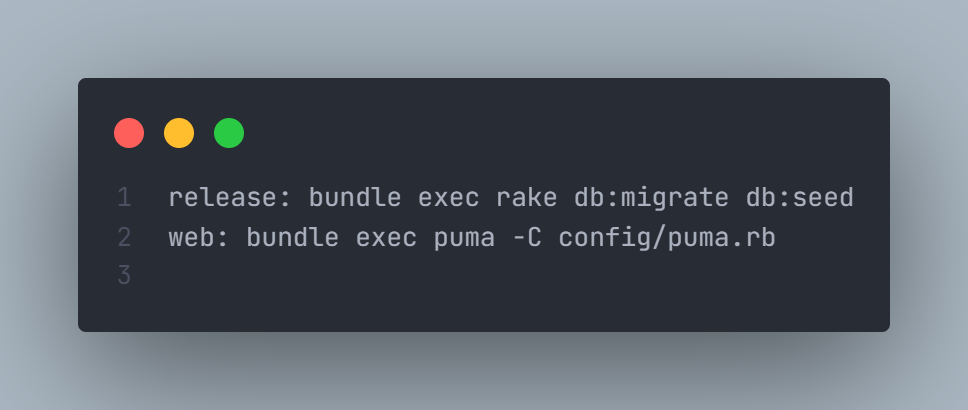
\includegraphics[width=150mm,scale=1]{figures/implementation_and_testing/deployment/image.png}}
        \caption{Procfile}
        \label{procfile}
    \end{figure}

    \clearpage
    \vspace{0.25cm}
    \newendline The Procfile is responsible for tailoring Heroku's default operation. Before releasing new versions, the commands "db:migrate" and "db:seed" are run with each new deployment to complete any outstanding migrations and seeds. This is done in preparation for deploying new versions. It is important to keep in mind that these instructions are disregarded if there is no need for migrations or seeds. The Puma web server, which is responsible for making the API available to users, is managed by the second section of the Procfile.

    \vspace{0.25cm}
    \newendline Heroku offers tools for monitoring the application, scaling it to manage greater traffic, and debugging any difficulties that may occur. The application may be viewed by going to a specific URL provided by Heroku which is the following link\newendline \href{https://stdc-api.herokuapp.com}{https://stdc-api.herokuapp.com}


    
\end{justify}
\clearpage


\subsection{Frontend Deployment (Client)}
\begin{justify}
    Render was used for the deployment of the frontend of the STDC Web Application, which was developed in React JS. Render is a comprehensive platform that provides an integrated solution for developing and operating applications and websites. It includes free SSL, a worldwide CDN, private networks, and automated deployments from Git.
    
    \vspace{0.25cm}
    \newendline The procedure for deployment on Render is really easy to understand. After committing the changes to the React application's GitHub repository, the application was linked to Render. Render was able to automatically recognize the Docker container that would be required to execute the React application and construct it. Render makes it possible for the client to supply any environment variables that are necessary before, during, or after the construction process. It is essential to keep in mind that React apps have the capability of consuming environment variables that are made accessible via the "REACT\_APP\_" prefix. The following is a list of environment variables that are utilized by the frontend.\\

    \renewcommand{\arraystretch}{1.0}
        \begin{longtable}[c]{|p{7.2cm}|p{7.2cm}|p{7.2cm}|p{7.2cm}|p{7.2cm}|}
        \caption{Environment Variables} \\
        \hline
        \textbf{Environment Variable} & \textbf{Description} \\
        \hline
        \endfirsthead
        \multicolumn{2}{c}%
        {\tablename\ \thetable\ -- \textit{Continued from previous page}} \\
        \hline
        \textbf{Environment Variable} & \textbf{Description} \\
        \hline
        \endhead
        \hline \multicolumn{2}{|c|}{\textit{Continued on next page}} \\ \hline
        \endfoot
        \hline
        \endlastfoot
        REACT\_APP\_DOMAIN & The Auth0 domain \\
        \hline
        REACT\_APP\_CLIENT\_ID & The Auth0 client ID \\
        \hline
        REACT\_APP\_AUDIENCE & The Auth0 audience \\
        \hline
        REACT\_APP\_API\_URL & The URL of the API \\
        \hline
        \end{longtable}


        \vspace{0.25cm}
        \newendline After the build was finished, the application was deployed, and a special Render URL was made available so that users could visit it. The application can be found on \newendline \href{https://stdc.onrender.com}{https://stdc.onrender.com}
        
        
        \newendline Render also includes tools for monitoring the program, reverting to older versions of the software, and debugging any problems that may occur.\\

        \vspace{0.25cm}
        \newendline To summarize, the deployment of the STDC Web Application demanded careful preparation and precise execution. A solution that is scalable, dependable, and easy to administer has been accomplished with the utilization of Heroku and Render for the deployment of the backend and frontend, respectively. The program may now be accessed by users, and its monitoring and maintenance can be done in a simple manner.


\end{justify}